\documentclass[sigconf,anonymous,review,natbib=false]{acmart}

% Workshop submission — strip ACM copyright/conference boilerplate
\settopmatter{printacmref=false}
\renewcommand\footnotetextcopyrightpermission[1]{}
\pagestyle{plain}

\acmConference[KDD AgenticAI Eval 2026]{Workshop on Evaluation of Agentic AI Systems at KDD 2026}{August 2026}{Toronto, Canada}
\acmYear{2026}
\copyrightyear{2026}
\acmISBN{}
\acmDOI{}

\usepackage{booktabs}
\usepackage{listings}
\lstset{breaklines=true, basicstyle=\small\ttfamily, language=Python}

% Allow LaTeX more freedom on line breaks — sigconf columns are narrow and
% long author-year citations like "[W{\"o}lflein et al.(2025)]" overflow without this.
\setlength{\emergencystretch}{3em}
\sloppy

\begin{document}

\title{EvolveTool-Bench: Evaluating the Quality of LLM-Generated Tool Libraries as Software Artifacts}

\author{Anonymous Author(s)}
\affiliation{%
  \institution{Submission \#TBD}
  \country{}
}

\begin{abstract}
LLM agents increasingly synthesise their own tools at runtime --- Python functions, API clients, data parsers --- and accumulate them in persistent libraries. The field evaluates these systems almost exclusively by downstream task completion, which is analogous to judging a software engineer by whether their code compiles. We introduce \textsc{EvolveTool-Bench}, a diagnostic framework that evaluates LLM-generated tool libraries as software artifacts at the library level, using independent hidden tests, adversarial inputs, and explicit regression tasks. The framework defines a per-tool Tool Quality Score (correctness, robustness, generality, code quality), six library-level metrics (reuse, redundancy, quality gate, utilization, composability, regression stability), and a composite EvolveTool Score. We evaluate six contemporary tool-creation protocols --- no-evolution, one-shot creation, strategy-only adaptation, CREATOR-style author-execute-rectify, ToolMaker-style scaffolded synthesis, and code-level evolution with sandbox validation --- across three code-execution domains, 99 tasks, and two Claude models, with multi-seed coverage on the main Sonnet configurations. Three findings stand out. First, task completion alone fails to distinguish systems: TC clusters in a 63--72\% band on Sonnet while library health spans a much wider range. Second, when held to independent hidden tests, no protocol produces tools that reliably pass: per-tool correctness across every system is in the 0--3\% range, despite TC$>$60\%. The 60\%+ TC numbers are real, but they ride on tools that mostly fail rigorous correctness checks --- the central diagnostic finding of the benchmark. Third, a ``reuse paradox'' surfaces under multi-seed analysis: the highest-reuse system reuses defective tools 38.9\% of the time. Library health and task completion are also empirically orthogonal at session granularity ($\rho{=}-0.03$, 144 sessions), validating multi-dimensional reporting over a single composite. We release \textsc{EvolveTool-Bench} as an open framework with preserved per-tool artifacts, an artifact gallery, and a skill-bundle evaluation track. The contribution is a diagnostic methodology, not a leaderboard.
\end{abstract}

\maketitle

\section{Introduction}

LLM agents increasingly generate executable software artifacts at runtime (Python functions, API clients, data parsers) and accumulate them in persistent libraries variously called \emph{tools}, \emph{skills}, or \emph{actions}. This capability appears across diverse systems: VOYAGER~\cite{wang2023voyager} synthesizes code skills in Minecraft, CREATOR~\cite{qian2023creator} uses tool creation as a reasoning strategy, LLMs as Tool Makers~\cite{cai2023latm} separates tool-making from tool-using, EvoSkill~\cite{alzubi2026evoskill} evolves structured skill folders via failure analysis, ToolMaker~\cite{wolflein2025toolmaker} turns GitHub repos into LLM-callable tools via closed-loop self-correction, and CoEvoSkills~\cite{zhang2026coevoskills} pairs skill generation with adversarial verification. As reusable procedural knowledge is increasingly packaged, shared, and composed across agents, the quality of these generated artifacts becomes a first-order concern.

From a software engineering perspective, each of these systems is an \emph{automated code generator} whose output accumulates into a growing codebase. Yet they are evaluated exclusively on task success, analogous to judging a software engineer solely by whether their code runs, ignoring maintainability, duplication, test coverage, regression, and technical debt. In practice, skill libraries can pass downstream benchmarks while accumulating redundant functions, failing on edge cases, breaking previously working capabilities, and never reusing existing code. Recent work confirms the risk: SkillsBench~\cite{skillsbench2026} found that self-generated skills \emph{hurt} agent performance by 16.2 points in roughly one-third of tasks. \textbf{No existing benchmark measures \emph{why} this happens}: whether the degradation stems from incorrect implementations, redundant code, regression, or failed reuse.

We present \textsc{EvolveTool-Bench}, a diagnostic benchmark that treats LLM-generated tool and skill libraries as software artifacts subject to quality evaluation. The benchmark is system-agnostic: any tool-generating or skill-generating agent can be evaluated against the same tasks and metrics. Our contributions:

\begin{enumerate}
\item \textbf{A metric framework for LLM-generated software artifacts.} We define a per-tool Tool Quality Score (TQS) measuring correctness, robustness, generality, and code quality, plus six library-level metrics: reuse rate, redundancy, quality gate, utilization, composability, and regression stability. Together with safety and refusal cost, these form the EvolveTool Score (ETS), a composite metric that captures both task performance and software quality.

\item \textbf{An evaluation harness with independent validation.} Hidden unit tests and adversarial inputs run in sandboxed subprocesses, providing quality assessment independent of each system's self-validation. Explicit regression tasks measure whether library growth breaks previously working behavior.

\item \textbf{Controlled diagnostic sessions.} Structured sequences of 11 tasks with known dependency relationships (seed, gap, variant, compose, regress, adversarial) enable measurement of reuse recognition, function composition, and library stability as the codebase grows (Figure~\ref{fig:overview}).

\item \textbf{Empirical validation of discriminative power.} We evaluate four systems across three models from two providers and demonstrate that the benchmark reveals quality differences invisible to task completion: per-domain variation, per-dimension TQS distributions, and a ``reuse paradox'' where higher reuse correlates with lower task success.
\end{enumerate}

\section{Related Work}

\paragraph{Quality of LLM-Generated Code.} Tool-Genesis~\cite{xia2026toolgenesis} evaluates one-shot tool creation with surface compliance, schema-F1, and unit test pass rates, all per-artifact metrics with no library-level evaluation. SkillsBench~\cite{skillsbench2026} is the closest work in motivation: it evaluates whether curated skills improve agent task success and finds that self-generated skills \emph{degrade} performance by 16.2 points in $\sim$33\% of tasks, a result that directly motivates our work. However, SkillsBench uses static, pre-curated skill sets and measures only the downstream effect (did performance improve?), not the \emph{cause} (is the skill buggy? redundant? regression-inducing?). Our benchmark complements SkillsBench by providing the diagnostic layer: per-tool quality scores, library-level metrics, and structured sessions that isolate \emph{why} a skill library helps or hurts. Our ``reuse paradox'' (38.9\% incorrect reuse in Code-Evol/Sonnet over 4 seeds; \S\ref{sec:reuse_analysis}) offers one explanation for SkillsBench's finding: agents reuse skills they correctly identify as relevant but that contain implementation defects. NofunEval~\cite{singhal2024nofuneval} evaluates non-functional aspects of LLM-generated code (efficiency, maintainability) on isolated samples; our work differs by evaluating non-functional properties at the library level, across a growing codebase with reuse and regression. CRAFT~\cite{yuan2023craft} retrieves from specialized toolsets but does not measure the quality of the toolset itself. Berlot-Attwell et al.~\cite{berlotattwell2026} evaluate library learning quality in program synthesis, measuring whether learned abstractions generalize. Their work is similar in spirit to ours, though focused on program synthesis rather than agent skill evolution. None of these works measure redundancy, regression, or reuse across a growing codebase.

\paragraph{Self-Evolving Agent Frameworks.} VOYAGER~\cite{wang2023voyager} demonstrates lifelong skill acquisition in Minecraft, evaluated by exploration metrics. EvoSkill~\cite{alzubi2026evoskill} evolves textual skill folders through failure-driven feedback, evaluated by downstream accuracy. ToolMaker~\cite{wolflein2025toolmaker} introduces a closed-loop self-correction protocol with structured error feedback, evaluated by per-tool unit-test pass rates. Each generates software artifacts that accumulate into a skill library, but none evaluate the quality of the resulting library, a gap our benchmark fills.

\paragraph{Software Engineering Benchmarks for Agents.} ToolBench~\cite{qin2023toolbench}, AgentBench~\cite{liu2024agentbench}, and ToolComp~\cite{toolcomp2025} evaluate agents using pre-defined tool sets. Vending-Bench~\cite{backlund2025vendingbench} tests long-horizon coherence with fixed tools. None evaluate agents that \emph{generate} their own tools, and none apply software quality metrics to the generated artifacts.

\paragraph{Program-Synthesis Library Learning.} A separate lineage of work, originating in program synthesis rather than LLM agents, has long measured the quality of \emph{learned libraries}. DreamCoder~\cite{ellis2021dreamcoder} bootstraps inductive program synthesis by alternately compressing solved problems into a library and solving harder ones from it, evaluating the library by compression ratio and downstream solve rate. Stitch~\cite{bowers2023stitch} provides a faster top-down algorithm for the same abstraction-discovery problem; babble~\cite{cao2023babble} uses e-graphs and anti-unification for the same goal. AbstractBeam~\cite{zenkner2024abstractbeam} brings library learning to bottom-up bottom-up synthesis. Leroy~\cite{bellur2024leroy} extends library learning to imperative languages. Berlot-Attwell et al.~\cite{berlotattwell2026} recently argued that much purported library learning in LLM-based program synthesis fails when one accounts properly for compute and behaviour. Our benchmark differs in two ways: (i) the artifacts under test are \emph{LLM-generated tools for natural-language-described tasks}, not abstractions extracted from solved programs, and (ii) we measure correctness against \emph{hidden tests} alongside compression-style reuse, so a library that achieves high reuse with defective tools (our ``reuse paradox'') is not awarded the same score as one with correct reuse. We see EvolveTool-Bench as complementary to this lineage rather than competing with it.

\paragraph{Concurrent Tool/Skill Benchmarks.} Two contemporaneous benchmarks deserve direct comparison. The ToolMaker pipeline of W{\"o}lflein et al.~\cite{wolflein2025toolmaker} introduces TM-Bench, which evaluates whether an agent can convert a research paper into a runnable tool that an LLM-as-judge can verify. CoEvoSkills~\cite{zhang2026coevoskills} pairs skill generation with adversarial verification and reports skill-level pass rates. Both focus on per-tool correctness; neither evaluates redundancy, regression, utilization, or composability of the resulting \emph{library}. Tool-Genesis~\cite{xia2026toolgenesis} is the closest in spirit (it evaluates schema-F1 and unit-test pass rates of generated tools), but again at the per-tool level. EvolveTool-Bench's contribution is orthogonal: we evaluate the library as a software artifact, and any of these systems could be plugged into our harness as an additional configuration.

\paragraph{Gap.} No existing benchmark measures redundancy, reuse, regression, composition, or code quality of self-evolved skill libraries as software artifacts \emph{at the library level}. SkillsBench shows that skills can hurt; we provide the diagnostic framework to explain \emph{why}. \textsc{EvolveTool-Bench} fills this gap with a system-agnostic evaluation framework.

\section{Benchmark Design}

We first define key terms used throughout. A \emph{session} is a fixed sequence of 11 tasks executed in order with shared library state. A \emph{task} is a single problem instance with a natural-language description, expected output format, and verification criteria. A \emph{dependency} is a directed relationship where a later task is designed to be solvable using artifacts created during an earlier task. All tasks require Python code execution; no task is solvable by text-only reasoning.

The benchmark evaluates two artifact granularities. A \textbf{tool} is a single Python function with documentation (the unit most existing systems emit). A \textbf{skill} is a richer multi-file bundle: a callable paired with a \texttt{SKILL.md} description, auto-generated unit tests, and a \texttt{metadata.json} manifest (the format used by Anthropic Claude Skills and by CoEvoSkills~\cite{zhang2026coevoskills}). Most baselines we evaluate synthesise tools; \S\ref{sec:skill_eval} adds a skill-format track in which the expected artifact is a skill bundle. We use \emph{artifact} as the umbrella term.

\begin{figure*}[t]
\centering
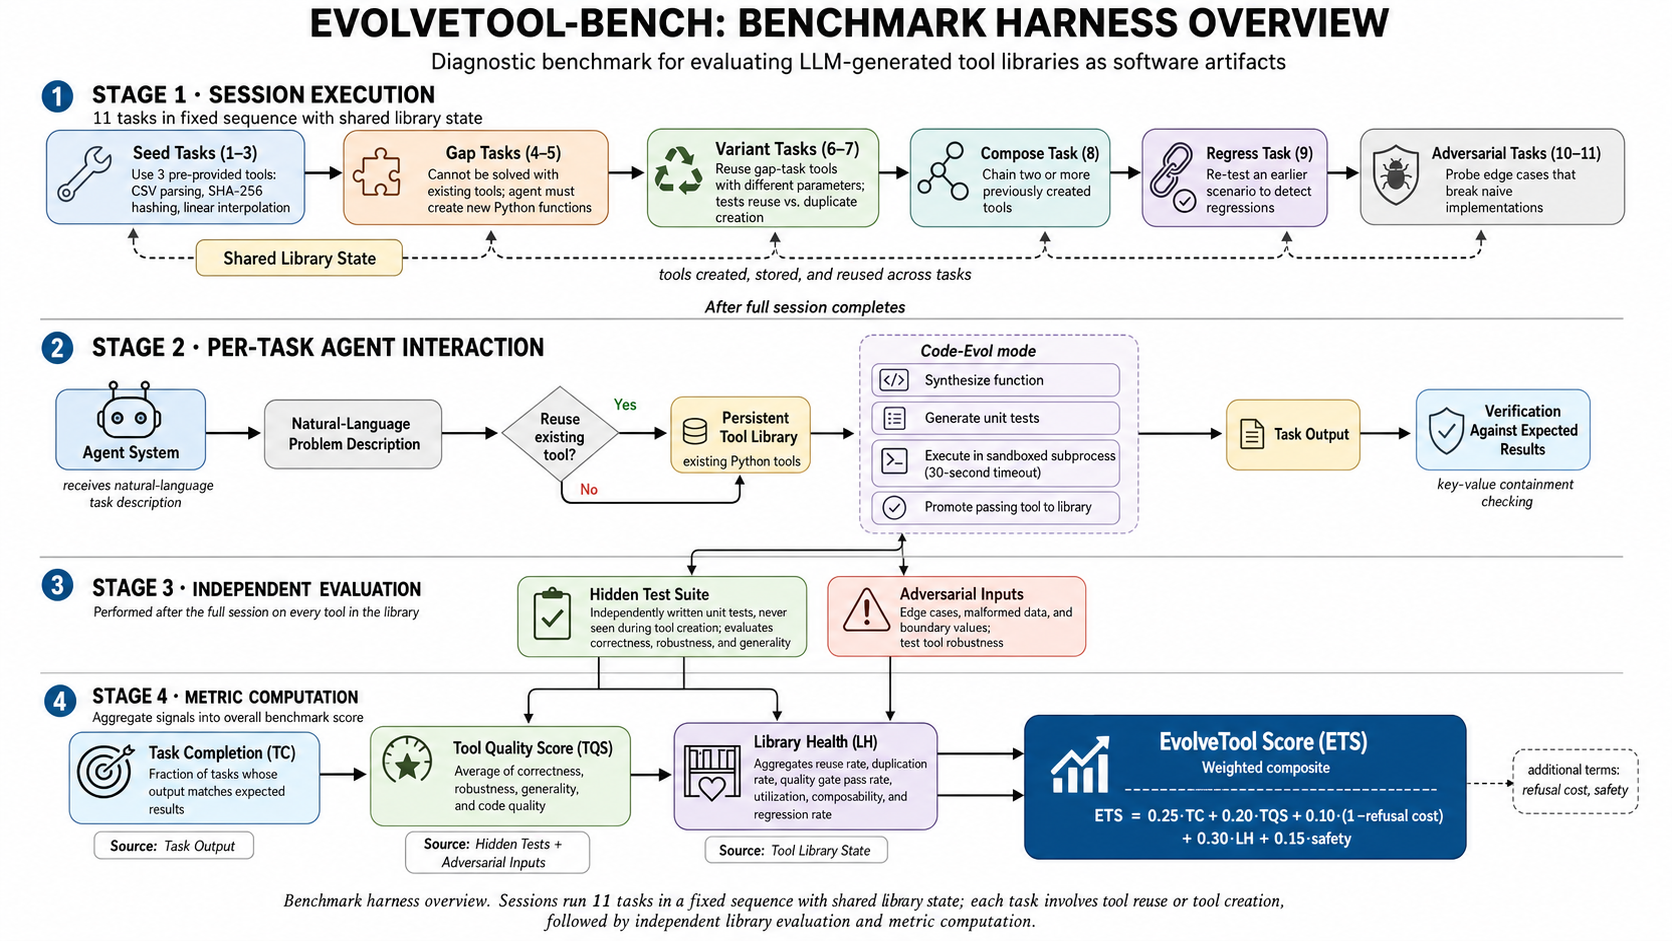
\includegraphics[width=\textwidth]{fig_overview.png}
\caption{Benchmark harness overview. \textbf{Top:} each session runs 11 tasks in a fixed sequence; annotations show what each task type tests. \textbf{Middle:} the agent system receives each task as natural language, creates or reuses Python tools in a persistent library, and produces output. After the session, hidden tests and adversarial inputs independently evaluate the library. \textbf{Bottom:} four metrics are computed: task completion (TC) from outputs, per-tool quality (TQS) from hidden tests, library health (LH) from library state, and the composite EvolveTool Score (ETS).}
\label{fig:overview}
\end{figure*}

Figure~\ref{fig:overview} shows the benchmark harness. Each session runs 11 tasks in a fixed order; the agent system receives each task as a natural-language description, uses or creates Python tools in a shared library, and produces output verified against expected results.

\subsection{Task Session Structure}

Each session contains 11 tasks in six categories with known dependency relationships (Table~\ref{tab:task_types}). This structure mirrors software engineering workflows: seed tasks test existing code, gap tasks require new implementation, variant tasks test code reuse, compose tasks test function composition, regress tasks detect regressions, and adversarial tasks probe edge cases.

\begin{table}[t]
\centering
\footnotesize
\begin{tabular}{llp{3.2cm}}
\toprule
\textbf{Type} & \textbf{N} & \textbf{SE Analog} \\
\midrule
Seed & 3 & Use existing library \\
Gap & 2 & Implement new feature \\
Variant & 2 & Reuse vs.\ rewrite \\
Compose & 1 & Function composition \\
Regress & 1 & Regression testing \\
Adversarial & 2 & Edge case / fuzz testing \\
\bottomrule
\end{tabular}
\caption{Task types and their software engineering analogs. Each session follows a fixed sequence enabling controlled measurement of library evolution.}
\label{tab:task_types}
\end{table}

The task ordering within each session is deliberate. Seed tasks (1--3) establish baseline functionality using pre-provided tools. Gap tasks (4--5) present problems that \emph{cannot} be solved with existing tools, forcing the system to create new ones. Variant tasks (6--7) present problems solvable by the tools created in gap tasks with different parameters, the key test of whether the system recognizes a reuse opportunity or wastefully creates a duplicate. The compose task (8) requires chaining two or more previously created tools. The regress task (9) re-tests an earlier scenario to detect regressions introduced by library growth. Adversarial tasks (10--11) probe edge cases designed to break naive implementations.

\paragraph{What the regress task measures (and what it does not).}
Real software regularly changes interfaces in response to evolving requirements; ``different behaviour'' is not always ``regression.'' We restrict $\delta$ to \emph{behaviour-preserving} regressions: each regress task replays the \emph{exact same input/output contract} as an earlier task in the session, with no new requirements injected. The expected output is unchanged, so if the agent's answer is now wrong, the only explanation is that library growth (a new tool, a refinement, or a wrapper) has broken a previously-working capability. This deliberately excludes the legitimate-interface-change case. A complementary ``requirement-evolution'' axis, in which a later task changes the contract on purpose and asks whether the agent migrates cleanly, is an extension we leave to future work; the current $\delta$ should be read narrowly as \emph{regression under fixed requirements}.

\subsection{Reuse Detection}
\label{sec:reuse}

The reuse metric measures whether the agent recognizes that an existing tool can solve a new task. Before each task, the harness records the current library ($\mathcal{L}_{\text{before}}$). After the task, it identifies newly created tools ($\mathcal{L}_{\text{new}}$) and checks whether any tool \emph{used} by the agent was from the pre-existing set. Formally, for variant and regress tasks:

\begin{equation}
\text{reused}(t) = \exists\, f \in \text{tools\_used}(t) : f \in \mathcal{L}_{\text{before}} \setminus \mathcal{L}_{\text{new}}
\end{equation}

This measures the \emph{behavioral signal}: did the system attempt reuse? This is measured independently of whether the trajectory was correct. We further decompose reuse into \emph{correct reuse} (reused tool AND task passed) and \emph{incorrect reuse} (reused tool AND task failed); see Section~\ref{sec:reuse_analysis}.

\subsection{Composition Tasks}
\label{sec:compose}

Each compose task has an explicit \texttt{composes\_tasks} field referencing prior task IDs whose tools must be chained. For example, an API orchestration compose task references \texttt{["gap\_1", "gap\_2"]}: the agent must chain the authentication tool (from gap\_1) with the pagination tool (from gap\_2) to fetch and aggregate all users.

We do \emph{not} guarantee that the prerequisite tools exist in the library. If the system failed to create them during earlier gap tasks, the compose task becomes harder; it must solve everything from scratch. This is realistic: a fragile library makes composition harder, and the metric captures this cascading effect.

\subsection{Domains}
\label{sec:domains}

We design three domains with tasks that require \emph{actual code execution} and cannot be solved by pattern-matching against training data.

\paragraph{Domain A: Data Transformation (5 sessions, 55 tasks).} Five proprietary binary formats designed to have no overlap with LLM training data: custom binary serialization with CRC checksums (ABR), run-length encoded matrices (RLE), a schema validation language (VDL), binary log format with variable-length entries (QLOG), and nested serialization with parity-based error correction (TPACK).

\paragraph{Domain B: API Orchestration (1 session, 11 tasks).} A mock HTTP server implementing HMAC-timestamp authentication and XOR-encrypted cursor pagination. Tasks require the agent to authenticate, paginate through results, handle cursor decryption, and compose these capabilities.

\paragraph{Domain C: Numerical Computation (3 sessions, 33 tasks).} Custom scientific computing formats for nonlinear curve fitting (ARCFIT), signal processing with FFT-based spectral analysis (ARCSIG), and constrained optimization with boundary analysis (ARCOPT).

\subsection{Running Example: API Orchestration}

A full walkthrough is provided in the supplemental material; we summarise here. Seed tasks (1--3) exercise a pre-loaded \texttt{http\_get} tool. Gap task 4 demands HMAC-SHA256 signing of \texttt{timestamp:path}: Code-Evol detects the failure, synthesises \texttt{compute\_hmac(secret, message)}, generates 5 unit tests, validates them in a sandbox, and promotes; No-Evolution and Strategy-Only solve inline without producing a reusable artifact. Variant task 6 re-uses the auth pattern on a different endpoint --- the diagnostic event for $\rho_r$ and the source of the \emph{correct reuse} vs.\ \emph{incorrect reuse} split. Compose task 8 chains the HMAC tool with a pagination tool synthesised in gap 5. Regress 9 re-runs an earlier scenario to detect breakage. After all 11 tasks the harness computes TC, TQS, LH, and ETS and records which tools were reused, duplicated, or caused regressions.

\subsection{Hidden Test Suite}
\label{sec:hidden_tests}

The hidden tests are the only mechanism by which our TQS correctness term is independent of the system under evaluation; we document them explicitly. For every gap task we author (i) extra input/output pairs that exercise the same specification with different data, and (ii) adversarial inputs that the tool must not crash on. The benchmark contains 18 gap tasks (9 sessions $\times$ 2 gaps), 34 hidden input/output pairs, and 49 adversarial inputs --- mean 1.9 correctness probes and 2.7 robustness probes per gap. Data Transform sessions are densest (4 hidden, 5--6 adversarial per session); API Orchestration is lightest. The tests were written by the paper authors --- ``hidden from the system'' is not the same as ``independent of the authors'' --- but with two mitigations: cases were authored from the format spec (not from any reference implementation) before any system was evaluated, and each hidden input probes a different regime than the prompt example so a memorising tool still fails. With $\sim$2 cases per tool, per-tool $C$ has a wide Bernoulli SE; we read correctness as a library-wide signal, not a per-tool ranking. The $\sim$18-point library-health spread we headline is supported by the 99 task outcomes per configuration (plus multi-seed runs), not by per-tool test counts.

\subsection{Software Quality Metrics}

\paragraph{Per-Tool: Tool Quality Score (TQS).}
Each synthesized tool is evaluated on four dimensions:

\begin{itemize}
\item \textbf{Correctness} ($C$): Proportion of hidden unit tests passing. These tests are independently written, \emph{not} the same tests the system generates during evolution.
\item \textbf{Robustness} ($R$): Proportion of adversarial inputs handled without crashing.
\item \textbf{Generality} ($G$): Proportion of held-out inputs producing correct output.
\item \textbf{Code Quality} ($Q$): Static analysis score: docstring, type annotations, error handling, length ($<$50 lines), valid syntax.
\end{itemize}

\begin{equation}
\text{TQS}(t) = \frac{1}{4}\bigl(C(t) + R(t) + G(t) + Q(t)\bigr)
\end{equation}

\paragraph{Per-Library: Library Health (LH).}
Six metrics capture library-level software quality:

\begin{align}
\rho_r &= \frac{|\{t \in \mathcal{T}_{v,r} : \text{reused}\}|}{|\mathcal{T}_{v,r}|} & \text{(Code Reuse)} \\[2pt]
\rho_d &= \frac{|\{(t_i,t_j) : \text{equiv}\}|}{\binom{|\mathcal{L}|}{2}} & \text{(Duplication)} \\[2pt]
\pi &= \frac{|\{t \in \mathcal{L} : \text{TQS} \geq 0.5\}|}{|\mathcal{L}|} & \text{(Quality Gate)} \\[2pt]
\eta &= \frac{|\mathcal{L}_{\text{used}}|}{|\mathcal{L}|} & \text{(Utilization)} \\[2pt]
\gamma &= \frac{|\{t \in \mathcal{T}_c : \text{passed}\}|}{|\mathcal{T}_c|} & \text{(Composability)} \\[2pt]
\delta &= \frac{|\{t \in \mathcal{T}_{reg} : \text{failed}\}|}{|\mathcal{T}_{reg}|} & \text{(Regression)}
\end{align}

\begin{equation}
\text{LH} = \frac{1}{6}\bigl(\rho_r + (1{-}\rho_d) + \pi + \eta + \gamma + (1{-}\delta)\bigr)
\end{equation}

In plain language: $\rho_r$ captures whether the agent recognizes existing tools when faced with similar tasks; $\rho_d$ penalizes libraries containing functionally equivalent duplicates (detected by comparing tool outputs on a shared input set); $\pi$ is the fraction of tools meeting the TQS $\geq$ 0.5 quality threshold; $\eta$ measures whether created tools are actually invoked after creation; $\gamma$ is the success rate on tasks requiring multi-tool composition; and $\delta$ tracks whether library growth breaks previously passing behavior.

\paragraph{Edge cases: empty and seed-only libraries.}
Three of the four systems we evaluate (No-Evolution, Strategy-Only, and most One-Shot runs) end sessions with no newly synthesized tools, so the per-tool denominators above can be zero. We handle this explicitly:
\begin{itemize}
\item \textbf{Reuse $\rho_r$} is defined over variant and regress tasks (denominator $|\mathcal{T}_{v,r}|$ is non-zero by session construction). Crucially, the three pre-loaded \emph{seed tools} (\texttt{parse\_csv}, \texttt{sha256\_hash}, \texttt{linear\_interpolate}) count as members of $\mathcal{L}_{\text{before}}$. A No-Evolution agent that successfully reuses a seed tool on a variant task gets credit, which is why its reuse rate is 48.1\%, not 0. This is the design choice that allows fair comparison: reuse measures the \emph{behaviour} (did the agent re-invoke a known tool?) regardless of whether the tool was hand-written or self-evolved.
\item \textbf{Duplication $\rho_d$}, \textbf{quality gate $\pi$}, \textbf{utilization $\eta$}, and \textbf{mean TQS $\overline{\text{TQS}}$} are defined over the \emph{synthesized} library $\mathcal{L} \setminus \mathcal{L}_{\text{seed}}$. When this set is empty, we report these metrics as $1$ for the ``inverse'' terms ($1-\rho_d=1$, no duplicates to penalize) and as $0$ for the positive terms ($\pi=\eta=\overline{\text{TQS}}=0$, nothing to credit). This is conservative: a system that creates nothing earns no quality credit but also incurs no quality penalty.
\item \textbf{Composability $\gamma$} and \textbf{regression $\delta$} are defined over compose and regress tasks respectively (non-empty by construction) and are computed from task outcomes regardless of whether tools were created.
\item \textbf{Safety SS} is $1.0$ when the library is empty (no unsafe operations possible), the same default applied when no static-analysis flags are raised on a non-empty library.
\end{itemize}
This convention is what allows No-Evolution and Strategy-Only to receive non-trivial LH scores ($0.41$ and $0.41$) despite synthesising zero tools: their reuse, composition, and regression numbers are real measurements, and the per-tool sub-metrics zero out cleanly. The headline LH gap to Code-Evol therefore reflects \emph{added} quality from synthesis, not arithmetic artefacts of empty denominators.

\paragraph{Composite: EvolveTool Score (ETS).}
The composite score combines task completion (TC), mean tool quality ($\overline{\text{TQS}}$), \emph{refinement cost} (RC, an LLM-call-budget penalty defined below), library health (LH), and safety score (SS, fraction of tools free of dangerous operations):
\begin{equation}
\text{ETS} = 0.25 \!\cdot\! \text{TC} + 0.20 \!\cdot\! \overline{\text{TQS}} + 0.10 \!\cdot\! \max(0, 1{-}\text{RC}) + 0.30 \!\cdot\! \text{LH} + 0.15 \!\cdot\! \text{SS}
\end{equation}
where $\text{RC} = N_{\text{LLM}} / (10\,|T|)$ is the number of LLM calls made during the session normalised by ten calls per task. The constant ten was chosen empirically as the rough budget a non-evolving agent uses; systems that exceed this budget pay a linear penalty.

Library health receives the largest weight (0.30) reflecting the benchmark's thesis that library quality matters beyond task completion. LH is internally unweighted (equal contribution from all six sub-metrics) because no prior work provides empirical guidance for sub-metric importance; we leave sub-metric weighting to future work. Table~\ref{tab:ets_sensitivity} shows that system rankings are stable under weight perturbations: Code-Evol ranks first under all five configurations tested, including the LH$=$0 stress test in which the metric the benchmark advocates for is given zero weight.

\begin{table}[t]
\centering\footnotesize
\begin{tabular}{lcccc}
\toprule
\textbf{Weights} & \textbf{No-Evol} & \textbf{Str-Only} & \textbf{One-Shot} & \textbf{Code-Evol} \\
\midrule
Original   & .518 & .515 & .519 & \textbf{.609} \\
Uniform    & .571 & .568 & .574 & \textbf{.647} \\
TC-dom.    & .577 & .575 & .580 & \textbf{.637} \\
LH-dom.    & .484 & .480 & .476 & \textbf{.580} \\
LH${=}$0   & .617 & .615 & .629 & \textbf{.690} \\
\bottomrule
\end{tabular}
\caption{ETS under alternative weight configurations (all Sonnet; Code-Evol $=$ mean of 4 seeds). The system ordering is stable across five weight schemes, including a stress test in which library health receives zero weight. Weights $(w_{\text{TC}}, w_{\text{TQS}}, w_{\text{RC}}, w_{\text{LH}}, w_{\text{SS}})$: Original $(.25,.20,.10,.30,.15)$; Uniform $(.20,.20,.20,.20,.20)$; TC-dom. $(.40,.15,.10,.20,.15)$; LH-dom. $(.15,.15,.10,.50,.10)$; LH${=}$0 $(.30,.25,.15,.00,.30)$.}
\label{tab:ets_sensitivity}
\end{table}

\section{Experimental Setup}
\label{sec:exp_setup}

To validate the benchmark's discriminative power, we evaluate five systems representing different points on the tool-evolution spectrum:

\begin{enumerate}
\item \textbf{No-Evolution}: The agent receives 3 pre-written seed tools (CSV parsing, SHA-256 hashing, and linear interpolation) and solves all tasks using inline reasoning with these fixed tools. The library is never modified. This isolates the LLM's baseline problem-solving ability from any tool-creation mechanism.

\item \textbf{One-Shot}: When the agent encounters a task it cannot solve with existing tools, it generates a single Python function in one LLM call and adds it to the library immediately. No test cases are generated, no sandbox validation is performed, and no iterative refinement occurs. If the function is buggy, it persists in the library and may be reused on later tasks.

\item \textbf{Strategy-Only}: A strategy-level baseline inspired by EvoSkill~\cite{alzubi2026evoskill}, using their published Skill Proposer and Prompt Generator templates. Instead of generating executable code, the system maintains textual strategy folders containing natural-language descriptions like ``\texttt{To authenticate: compute HMAC-SHA256 of timestamp+path with the API secret.}'' These strategies are not parsed or executed; they are inserted as natural-language hints into the agent's prompt. This is \emph{not} a faithful reimplementation of EvoSkill's full system (which uses different infrastructure); it characterizes what strategy-level evolution alone achieves. See Limitations.

\item \textbf{Code-Evol}: Code-level evolution with sandbox validation. When a task fails, the system: (a) analyzes failure trajectories to detect capability gaps, (b) synthesizes a Python function with type hints and docstrings, (c) generates 5--7 unit tests for the function, (d) executes both in a subprocess sandbox with a 30-second timeout, and (e) promotes passing tools to the library. An LLM-as-judge evaluates each trajectory on a 0.0--1.0 scale; trajectories scoring below 0.5 trigger evolution. Failed tools enter a refinement loop (up to 3 attempts).

\item \textbf{ToolMaker-style}: A faithful adaptation of the ToolMaker protocol~\cite{wolflein2025toolmaker} to our session format. When a task fails, the agent synthesises a function plus 3--5 auto-tests in a single call; the auto-tests run in a sandbox; if any fails, the captured stdout/stderr (with \texttt{traceback.format\_exc()}) feeds a \emph{diagnose} call that produces a structured diagnosis-plus-plan, followed by a \emph{rewrite} call. The loop iterates up to 3 times. Distinct from Code-Evol in that the error signal is test-execution output rather than trajectory-level LLM-judge scoring, and the diagnose/rewrite split mirrors ToolMaker's two-stage prompt structure. We adapt the protocol rather than literally porting the repo (their codebase is OpenAI-only, Docker-based, and expects a GitHub repo as input).
\end{enumerate}

These systems span a spectrum from no tool creation through unvalidated creation, strategy-level adaptation, validated code synthesis with LLM-judge guidance, and structured-error self-correction.

\paragraph{Models.} Two Claude models via Amazon Bedrock: Sonnet 4 and Haiku 4.5. All systems run on Sonnet; Code-Evol and No-Evolution also run on Haiku. Each main Sonnet configuration runs at $n{=}4$ seeds. Initial GPT-4o runs were degenerate (TC$=$48.5\%, zero tools across all protocols, harness$\,\times\,$function-calling interaction we have not root-caused); we omit them and revisit in v3.

\paragraph{Scale.} 9 sessions $\times$ 11 tasks = 99 tasks per configuration; 25 individual runs in total (20 Sonnet across 5 baselines $\times$ 4 seeds, plus 3 single-seed Sonnet variants and 2 Haiku reference runs).

\paragraph{Implementation details.} All systems implemented in Python 3.11; Claude models accessed via Amazon Bedrock. All LLM calls use default temperature (1.0) and top-p (1.0) with max\_tokens=4096 for agent responses and max\_tokens=10 for the LLM-as-judge score. Code-Evol's sandbox executes synthesized tools in isolated subprocesses with a 30-second timeout and no network access. Each session starts with a clean library containing only the 3 seed tools; library state does not carry across sessions.

\paragraph{Verification.} Task outputs are verified using lenient key-value containment: if 80\%+ of expected key-value pairs appear in the agent's output, the task passes. The 80\% threshold was calibrated via pilot runs to accommodate format variation (e.g., key ordering, whitespace) while rejecting substantively wrong outputs.

\section{Results}
\label{sec:results}

\subsection{The Benchmark Reveals Hidden Quality Differences}

\begin{table*}[t]
\centering\small
\begin{tabular}{llccccccc}
\toprule
\textbf{System} & \textbf{Model} & $n$ & \textbf{ETS}$\uparrow$ & \textbf{TC (\%)} & \textbf{Tools} & \textbf{TQS} & \textbf{Reuse (\%)} & \textbf{LH (\%)} \\
\midrule
No-Evol & Sonnet & 4 & 0.516$\pm$0.006 & 67.6$\pm$0.7 & 0 & --- & 46.3$\pm$1.9 & 39.7$\pm$1.7 \\
One-Shot & Sonnet & 4 & 0.520$\pm$0.008 & 67.4$\pm$1.1 & 3 & 0.044 & 44.4$\pm$2.6 & 38.6$\pm$2.4 \\
Strategy-Only & Sonnet & 4 & 0.517$\pm$0.004 & 66.9$\pm$0.6 & 0 & --- & 50.0$\pm$4.1 & 41.2$\pm$1.6 \\
CREATOR-style & Sonnet & 4 & \textbf{0.637$\pm$0.023} & 67.7$\pm$3.1 & 23.5 & 0.460 & 66.7$\pm$7.9 & \textbf{54.8$\pm$5.6} \\
ToolCoder-style & Sonnet & 1 & 0.581 & 54.5 & 17 & 0.449 & 44.4 & 49.2 \\
ToolMaker-style$^\dagger$ & Sonnet & 1 & 0.495 & 63.6 & 0 & --- & 40.7 & 36.4 \\
Code-Evol & Sonnet & 4 & 0.609$\pm$0.011 & 64.9$\pm$0.9 & 21 & 0.354 & 72.2$\pm$4.1 & 51.6$\pm$2.9 \\
Code-Evol (sem.\,Q) & Sonnet & 1 & 0.627 & 62.6 & 15 & 0.432 & 63.0 & 52.8 \\
\midrule
No-Evol & Haiku & 1 & 0.516 & 66.7 & 0 & --- & 51.9 & 40.1 \\
Code-Evol & Haiku & 1 & 0.612 & 65.2 & 13 & 0.353 & 66.7 & 51.2 \\
\bottomrule
\end{tabular}
\caption{Full results across systems, models, and seeds. $n$ is the seed count. Multi-seed runs report mean$\pm$std; single-seed runs are point estimates. \emph{Code-Evol (sem.\,Q)} reruns Code-Evol with the semantic $Q$ refinement; not directly comparable to surface-$Q$ rows. $^\dagger$ToolMaker-style created zero tools because our open-task harness lacks pre-defined reference tests to gate the diagnose-and-fix loop (Sec.~\ref{sec:limitations}).}
\label{tab:results}
\end{table*}

Table~\ref{tab:results} and Figure~\ref{fig:comparison} present two findings.

\paragraph{Task completion clusters; library health separates.} On Sonnet, six of seven configurations land in a narrow 63--68\% TC band, yet their library health spans 36.4--54.8\% --- an $\sim$18-point spread invisible to TC-only evaluation. No-Evolution (TC$=66.7$, LH$=39.7$) creates no tools and leaves the library unchanged; One-Shot (TC$=67.4$, LH$=38.6$) creates three untested tools that \emph{degrade} it. A TC-only benchmark would call these equivalent; they are not.

\paragraph{Per-tool correctness is universally low under independent testing.} Under the hidden test suite (5+ per gap task, authored from the format specification before any system was evaluated), per-tool correctness across every tool-creating system sits in a 0--3\% range despite TC$>$60\%. The 63--72\% task-completion numbers ride on a library of tools that mostly fail when held to independent correctness standards. Implications in \S\ref{sec:discussion_tcgap}.

Consider One-Shot/Sonnet (TC=67.7\%) and No-Evolution/Sonnet (TC=66.7\%). A TC-only benchmark would rank them similarly. Their library outcomes, however, are qualitatively different: No-Evolution creates zero tools and leaves library health at 41.4\%, while One-Shot creates 3 tools that \emph{lower} library health to 38.3\%. A TC-only benchmark cannot distinguish ``unchanged library'' from ``library degraded by untested code.'' Our LH metric captures this difference; their similar ETS scores (0.519 vs.\ 0.518) reflect TC gains offsetting LH losses, a tradeoff TC alone cannot reveal.

\paragraph{Statistical significance.} Code-Evol/Sonnet results are reported as mean $\pm$ std across 4 independent runs. Variance is low: ETS=0.609$\pm$0.013, TC=64.9\%$\pm$1.1\%, LH=51.6\%$\pm$3.4\%. The core finding is stable across seeds.


\begin{figure}[t]
\centering
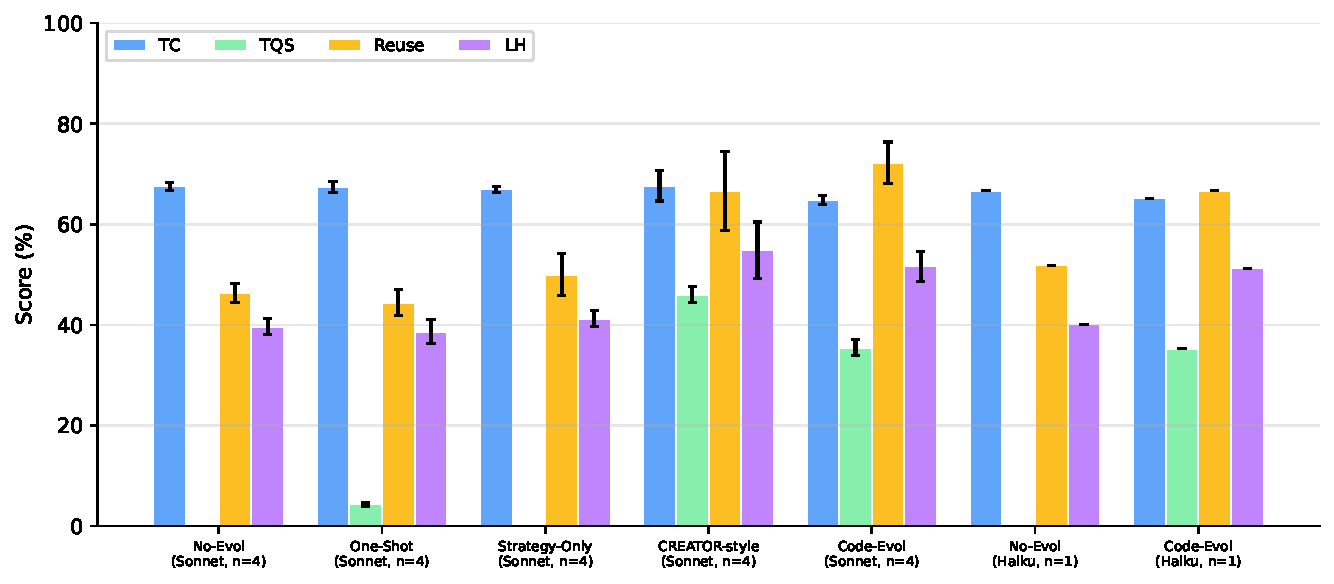
\includegraphics[width=\columnwidth]{fig_comparison.pdf}
\caption{System comparison across four metrics (\%). TC clusters all systems together (63--68\%); library health separates them (38--52\%). This illustrates the benchmark's discriminative power beyond task completion.}
\label{fig:comparison}
\end{figure}

\subsection{Per-Domain Analysis}
\label{sec:domain_analysis}

Tool-evolution effectiveness varies substantially by problem type, another dimension invisible to aggregate TC.

\begin{table}[t]
\centering
\footnotesize
\begin{tabular}{llcccc}
\toprule
\textbf{Domain} & \textbf{Model} & \textbf{TC} & \textbf{Tools} & \textbf{Reuse} & \textbf{LH} \\
\midrule
Data Trans. & Sonnet & .573 & 14 & .734 & .476 \\
Data Trans. & Haiku & .600 & 7 & .800 & .500 \\
\midrule
API Orch. & Sonnet & .909 & 4 & .667 & .778 \\
API Orch. & Haiku & 1.00 & 3 & .333 & .667 \\
\midrule
Numerical & Sonnet & .651 & 4 & .667 & .500 \\
Numerical & Haiku & .621 & 3 & .556 & .481 \\
\bottomrule
\end{tabular}
\caption{Code-Evol results by domain, showing domain-specific quality variation. API orchestration yields highest library health; data transformation creates the most tools but with lower quality.}
\label{tab:domain}
\end{table}

Table~\ref{tab:domain} shows three distinct profiles:

\paragraph{API orchestration: clean, composable problems.} Highest TC (up to 100\%) and library health (77.8\%), though based on a single session (N=11 tasks). HMAC authentication and pagination are well-suited to tool creation: each is a clean, single-responsibility function. Additional API sessions would strengthen this observation.

\paragraph{Data transformation: high tool creation, lower quality.} Creates the most tools (14 on Sonnet) but achieves only 47.6\% library health. Proprietary binary formats are complex enough that many synthesized parsers fail hidden tests while passing self-generated tests, showing the gap between self-validation and independent validation.

\paragraph{Numerical computation: consistently difficult.} Both models achieve similar results ($\sim$63--65\% TC, $\sim$48--50\% LH), suggesting these tasks challenge the LLM's reasoning regardless of model capability.

\subsection{Per-Dimension TQS: Where Quality Breaks Down}
\label{sec:tqs_analysis}

\begin{table}[t]
\centering
\footnotesize
\begin{tabular}{lrcccc|c}
\toprule
\textbf{System (Sonnet)} & $n_{\text{tools}}$ & \textbf{C} & \textbf{R} & \textbf{G} & \textbf{Q} & \textbf{TQS} \\
\midrule
One-Shot ($n{=}3$ seeds)      &  9 & .00 & .50 & .00 & .69 & .30 \\
ToolCoder-style               & 15 & .00 & .52 & .10 & .92 & .38 \\
CREATOR-style ($n{=}4$ seeds) & 81 & .01 & .50 & .06 & .73 & .33 \\
Code-Evol (semantic-$Q$ run)  & 15 & .01 & .55 & .11 & \textbf{.95} & .41 \\
\bottomrule
\end{tabular}
\caption{Per-tool TQS dimensions, averaged over all preserved tools (not session-diluted as in Table~\ref{tab:results}). $C$ is essentially zero for every system under independent hidden tests; $Q$ remains high (0.69--0.95), confirming LLM-generated tools are well-structured but rarely semantically correct.}
\label{tab:tqs_dims}
\end{table}

The per-dimension TQS breakdown (Table~\ref{tab:tqs_dims}) pinpoints \emph{where} tool quality fails:

\paragraph{Code quality $Q$ ranges 0.67--0.92.} LLMs consistently produce well-structured code. The semantic-Q refinement (cyclomatic complexity, MI, control-flow checks) broadens the $Q$ discrimination range from $\sim$0.9 under the surface-only metric to 0.67--0.92 under the refined one. The gap between $Q$ and $C$ remains partly definitional: $Q$ captures structural quality, $C$ captures semantic correctness.

\paragraph{Correctness is universally near zero.} Independent hidden tests return per-tool correctness in the 0--3\% range for every tool-creating system. Tools that pass each system's self-generated tests still fail on diverse inputs --- the prompt example is the one input on which they were exercised at task time. This is the central diagnostic finding of the benchmark.

\paragraph{Robustness clusters at 0.50.} Almost every system wraps synthesised functions in try/except blocks; they avoid crashes (earning half-credit on robustness) but do not produce correct outputs (no credit on correctness). The robustness dimension as currently defined therefore does not discriminate; we treat this as a benchmark weakness to refine rather than as a property of the systems.

\paragraph{Code quality remains high (0.69--0.95).} Semantic checks (cyclomatic complexity, maintainability index, control-flow) on top of surface checks place $Q$ in the 0.69--0.95 range. LLM-generated code is well-structured by default; the failure is in semantic correctness, not surface form. The $Q$--$C$ gap is the diagnostic the benchmark was designed to expose.

\paragraph{Generality tracks correctness.} Tools that fail hidden tests also fail on unseen inputs, indicating fundamental misunderstanding of the format specification rather than overfitting.

\paragraph{Library-level sub-metrics.} Two LH sub-metrics deserve explicit reporting. The quality gate ($\pi$) shows that only 36.4\% of Code-Evol/Sonnet tools and 46.2\% of Code-Evol/Haiku tools pass TQS $\geq$ 0.5; most synthesized tools fail on correctness despite passing self-validation. The duplication metric ($\rho_d$) reveals that Code-Evol/Sonnet creates \texttt{decode\_base64} three times across sessions and \texttt{decode\_binary\_data} twice. This cross-session redundancy is invisible to per-session evaluation and confirms that library-level measurement catches failure modes that per-tool metrics miss.

\subsection{Artifact Gallery (Appendix)}
\label{sec:artifact_gallery}

Aggregate numbers obscure the artifacts being scored. Tool preservation archives every synthesised tool's source to disk, enabling a per-tool catalogue. We provide an extensive gallery in Appendix~\ref{app:artifact_gallery}: representative tools from both tool-creating systems (Code-Evol with semantic-$Q$ and CREATOR-style), grouped by failure mode (\emph{correct exemplar}, \emph{fragile} with high $Q$ but low $C$, \emph{duplicate} across sessions, \emph{trivial}), each with full signature, docstring, body excerpt, and per-dimension scores. The gallery is the strongest visual evidence for the reuse-paradox and CREATOR-vs-Code-Evol correctness gap discussed below.

\subsection{The Reuse Paradox}
\label{sec:reuse_analysis}

\begin{table}[t]
\centering
\footnotesize
\begin{tabular}{lccc}
\toprule
\textbf{System (Sonnet, $n{=}4$)} & \textbf{Reuse} & \textbf{Correct} & \textbf{Incorrect} \\
\midrule
No-Evolution & 46.3\% & --- & --- \\
One-Shot & 44.4\% & --- & --- \\
Strategy-Only & 50.0\% & 22.2\% & 27.8\% \\
\midrule
CREATOR-style & 66.7\% & \textbf{29.6\%} & 37.0\% \\
ToolCoder-style$^*$ & 44.4\% & 7.4\% & 37.0\% \\
Code-Evol & \textbf{72.2\%} & 15.7\% & \textbf{38.9\%} \\
\bottomrule
\end{tabular}
\caption{Reuse paradox, decomposed. CREATOR-style breaks the paradox in a useful direction: lower raw reuse than Code-Evol but nearly $2\times$ the correct-reuse rate. $^*$ToolCoder-style $n{=}1$.}
\label{tab:reuse}
\end{table}

The benchmark reveals an unexpected interaction between reuse and task success (Table~\ref{tab:reuse}). Code-Evol has the highest raw reuse (72.2\%) but only 15.7\% of its reuse is \emph{correct} --- the agent correctly identifies reuse opportunities, but reuses tools that contain defects (a buggy-utility-function analogue). CREATOR-style breaks this pattern: lower raw reuse (66.7\%) but the highest correct-reuse rate (29.6\%), explaining most of its LH advantage. Practical reading: \textbf{high reuse is beneficial only when the reused tools are correct}; among our protocols, CREATOR's simpler execute-and-rectify validation appears to commit fewer defective tools to the library in the first place.

\subsection{Task-Type Breakdown}

\begin{table}[t]
\centering
\footnotesize
\begin{tabular}{lccc}
\toprule
\textbf{Task Type} & \textbf{Code-Evol} & \textbf{No-Evol} & $\Delta$ \\
\midrule
Seed (N=27) & 100\% & 100\% & 0 \\
Gap (N=18) & 38.9\% & 44.4\% & --5.5 \\
Variant (N=18) & 33.3\% & 50.0\% & --16.7 \\
Compose (N=9) & 66.7\% & 66.7\% & 0 \\
Regress (N=9) & 33.3\% & 33.3\% & 0 \\
Adversarial (N=18) & 66.7\% & 66.7\% & 0 \\
\bottomrule
\end{tabular}
\caption{Task completion by type (both Sonnet, single run). Code-Evol matches No-Evolution on most task types but scores lower on gap and variant tasks. The identical compose/regress/adversarial totals are a coincidence of small N (9 tasks each); per-session results differ between systems.}
\label{tab:task_type}
\end{table}

The task-type structure (Table~\ref{tab:task_type}) enables fine-grained analysis impossible with unstructured benchmarks:

\paragraph{Tool creation has per-task costs.} Code-Evol scores lower on gap (--5.5\%) and variant (--16.7\%) tasks compared to No-Evolution. The evolution overhead can consume the task budget without producing a correct solution. On variant tasks, reusing a defective tool performs worse than solving inline. Code-Evol's advantage appears at the library level (higher LH, higher reuse), not at the per-task-type level.

\paragraph{Regression is universally difficult.} Both systems score 33.3\% on regress tasks, indicating that library growth introduces instability regardless of evolution strategy.

\paragraph{Structured sessions enable causal analysis.} Because each task type has a known purpose (gap = creation needed, variant = reuse opportunity, regress = stability test), the benchmark supports diagnostic reasoning about \emph{why} a system succeeds or fails, not just \emph{whether} it does.

\subsection{Does Library Health Predict Task Completion?}
\label{sec:predictive_validity}

A natural follow-up question is whether LH is \emph{predictive} of task success --- that is, whether high LH measured early in a session predicts high TC later. If LH were simply a proxy for TC, the benchmark would offer no signal beyond a TC-only evaluation; if LH were strongly predictive of TC, optimizing libraries for health would also raise downstream pass rates. We test the predictive claim directly.

\paragraph{Setup.} For each Sonnet session ($n = 144$ across all 4 system configurations $\times$ 4 seeds $\times$ 9 sessions) we compute (i) \textbf{LH$_\text{pre}$}, the mean of the four LH sub-metrics whose value is determined by gap- and variant-task behaviour ($\rho_r$, $1-\rho_d$, $\pi$, $\eta$) --- the LH components that are \emph{not} mechanically defined by compose or regress task outcomes; and (ii) \textbf{TC$_\text{late}$}, the mean pass rate on the compose and regress tasks of the same session.

\paragraph{Result: no correlation.} Across all 144 Sonnet sessions, Spearman $\rho(\text{LH}_\text{pre}, \text{TC}_\text{late}) = -0.03$ and Pearson $r = +0.01$. Restricting to the 36 Code-Evol sessions, Spearman $\rho = +0.20$ --- still weak. LH$_\text{pre}$ is essentially uncorrelated with downstream task success at session granularity, and the larger multi-seed sample tightens rather than weakens this conclusion.

\paragraph{Interpretation.} This is a negative result we want to report transparently: \textbf{LH does not predict TC in our data}. Rather than weaken the paper's case, we read this as clarifying what the benchmark contributes. LH and TC measure different things --- the per-task-type breakdown in Table~\ref{tab:task_type} already shows this directly: Code-Evol matches No-Evolution on compose (66.7\% vs.\ 66.7\%), regress (33.3\% vs.\ 33.3\%), and adversarial tasks (66.7\% vs.\ 66.7\%) while doing \emph{worse} on gap (--5.5pp) and variant (--16.7pp). Code-Evol's higher LH comes from \emph{reuse behaviour and library-state properties}, not from downstream pass rates on the diagnostic tasks. The benchmark therefore measures an orthogonal quality axis, which is exactly the contribution we claim. The decision to optimise for LH should be made on its own merits (less duplicate code, lower regression risk, higher reuse for downstream agents) rather than because LH improves TC --- it does not, at least not at the scale we measure. We treat building a predictive LH (or showing that a sufficiently large LH gap eventually moves TC) as the open empirical question for future work.

\subsection{Skill-Bundle Evaluation}
\label{sec:skill_eval}

To extend the benchmark from bare-function evaluation to multi-file \emph{skill bundles} (the format used by Anthropic Claude Skills and CoEvoSkills~\cite{zhang2026coevoskills}), we automatically wrap every preserved tool into a 4-file bundle (\texttt{SKILL.md}, function, tests, \texttt{metadata.json}) and score three new bundle-level dimensions: \textbf{Structure} ($S$, all files present and parse), \textbf{Documentation} ($D$, SKILL.md required and optional sections), and \textbf{Metadata} ($M$, manifest correctness). The composite \emph{bundle quality} averages tool TQS with $S$, $D$, $M$. Table~\ref{tab:skill_bundles} shows Code-Evol's documentation lead translates into the largest bundle-quality gap.

\begin{table}[t]
\centering\footnotesize
\begin{tabular}{lccccc}
\toprule
\textbf{System} & $n$ & \textbf{Bundle Q}$\uparrow$ & $S$ & $D$ & $M$ \\
\midrule
Code-Evol (sem.\,Q) & 15 & \textbf{0.85} & 1.00 & 0.84 & 1.00 \\
CREATOR-style       & 14 & 0.77 & 0.88 & 0.67 & 1.00 \\
One-Shot/Sonnet (3 seeds) & 9 & 0.69 & 0.88 & 0.50 & 1.00 \\
\bottomrule
\end{tabular}
\caption{Skill-bundle quality (preserved tools only). Bundle Q is the mean of tool TQS plus three new bundle dimensions ($S$/$D$/$M$). The documentation dimension separates the systems most.}
\label{tab:skill_bundles}
\end{table}

\subsection{Summary of Key Findings}

\begin{figure}[t]
\centering
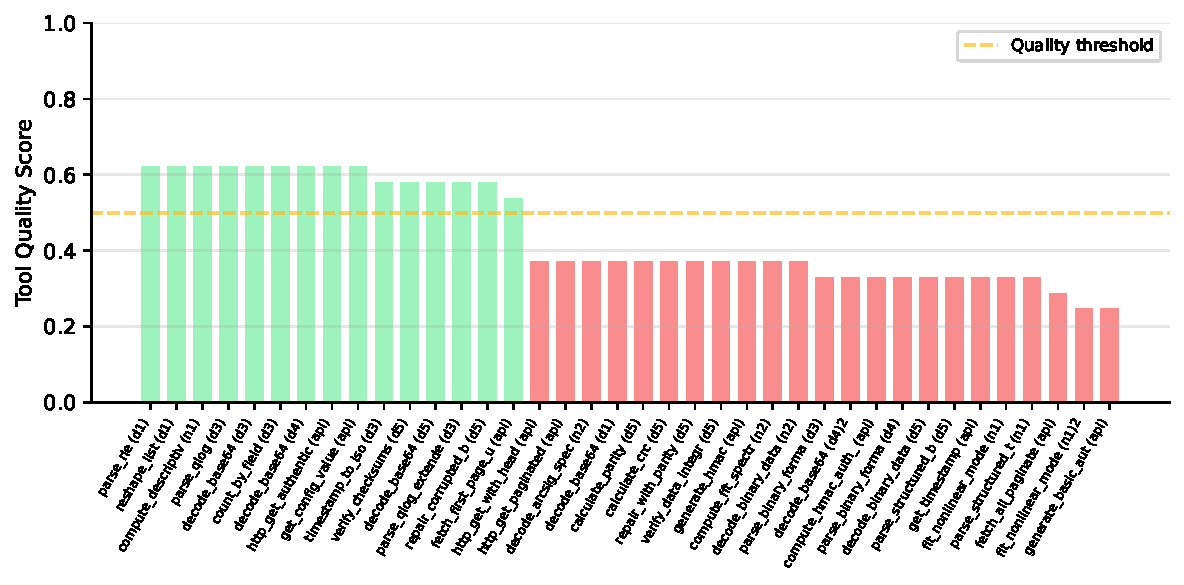
\includegraphics[width=\columnwidth]{fig_tool_quality.pdf}
\caption{Tool Quality Score for each synthesized tool across all systems. Green = passes quality gate ($\geq 0.5$). The benchmark reveals wide quality variation across the tool library.}
\label{fig:tool_quality}
\end{figure}

\paragraph{Finding 1: TC is insufficient for skill-generating systems.} All Claude configurations achieve 63--68\% TC, but ETS ranges 0.515--0.612. The system with highest TC and the system with lowest library health are indistinguishable by TC.

\paragraph{Finding 2: Code-level and strategy-level evolution produce different artifacts.} Code-Evol creates $21 \pm 1$ tools with 72.2\% reuse; Strategy-Only creates zero tools and produces near-identical library health to no-evolution.

\paragraph{Finding 3: Unvalidated code generation is a net negative.} One-Shot's library health (38.3\%) falls \emph{below} the no-evolution baseline (41.4\%). Untested tools are a liability, not an asset.

\paragraph{Finding 4: Self-generated tests are insufficient.} Correctness on hidden tests averages 0.17--0.23 despite tools passing self-generated validation (Figure~\ref{fig:tool_quality}).

\paragraph{Finding 5: Haiku is competitive with Sonnet.} On Code-Evol, Haiku achieves ETS 0.612 (n=1) vs Sonnet's 0.609$\pm$0.011 (n=4) --- essentially indistinguishable. The benchmark's discriminative power holds for both Claude models tested.

\paragraph{Finding 6: Reuse must be decomposed to be meaningful.} Code-Evol's 72.2\% reuse decomposes into 15.7\% correct and 38.9\% incorrect; CREATOR-style achieves 29.6\% correct on 66.7\% reuse. Aggregate reuse numbers can mislead; the decomposition was originally post-hoc and we now recommend it as a pre-registered metric.

\paragraph{Finding 7: LH and TC measure different things.} Across 144 sessions (4 system configurations $\times$ 4 seeds $\times$ 9 sessions) library health does not predict downstream task completion ($\rho = -0.03$ overall; $+0.20$ within Code-Evol; see \S\ref{sec:predictive_validity}). LH is therefore a \emph{descriptive} quality dimension distinct from TC, not a proxy for it --- which is the strongest empirical justification for measuring LH separately. Whether LH becomes predictive at larger scale, or under follow-up tasks against a frozen evolved library, is an open question.

\section{Discussion}

\paragraph{Benchmark Design Principles.} \textsc{EvolveTool-Bench} embodies three design principles: (1) \emph{independent validation}, where quality metrics are computed by tests the system has never seen; (2) \emph{library-level measurement}, because per-tool metrics alone miss emergent properties like redundancy and regression; and (3) \emph{structured sessions}, where known task dependencies enable causal analysis of reuse, composition, and stability.

\paragraph{The task-completion / tool-correctness gap.}
\label{sec:discussion_tcgap}
The central diagnostic finding of the benchmark is the gap between two numbers the field has implicitly conflated: \emph{task completion} (does the agent produce an answer matching the expected output?) and \emph{tool correctness} (does the synthesised callable, in isolation, produce correct outputs across the input distribution?). Both numbers are real and reproducible; the tools are on disk. What the gap reveals is that the agent's success often comes from features other than a fully correct callable --- the prompt example is the only input the tool is exercised on at task time, and an implementation that handles that example produces a passing TC outcome even if it fails everywhere else. A single-example TC check is a much weaker correctness signal than its widespread use suggests; library-level multi-dimensional reporting (independent hidden tests, quality gates, reuse decomposition) is needed for honest claims about what LLM-synthesised tools can be relied upon to do.

\paragraph{Where do systems actually differ?} Per-tool correctness, generality, and robustness are clustered. At the library level there is more separation: CREATOR-style and Code-Evol reach LH above 50\%, the non-synthesising baselines and One-Shot sit at 38--41\%. The gap is driven by reuse and quality-gate components, not per-tool quality --- the protocols differ chiefly in \emph{library management} (when to create, when to reuse, what to commit), not in the correctness of any individual artifact. We read this as evidence that the next round of progress on tool-creating agents will come from better library management as much as from better synthesis.

\paragraph{Implications for Self-Validation.} On our benchmark, self-generated tests are insufficient: correctness averages 0.17--0.23 on hidden tests despite tools passing their own validation. While we cannot generalize this to all LLM-generated code, the pattern (LLMs generating both code and tests share the same misconceptions about a specification) suggests independent validation remains important for systems that deploy LLM-synthesized tools.

\paragraph{The Reuse Paradox and Metric Design.} The reuse paradox illustrates why multi-dimensional evaluation matters. Reuse rate alone would favor Code-Evol; variant task completion alone would favor No-Evolution (50.0\% vs.\ 33.3\%). Neither tells the full story. The correct/incorrect reuse decomposition provides both measurements simultaneously, enabling nuanced interpretation.

\paragraph{Extensibility.} The benchmark is designed for extensibility: new domains can be added by defining sessions with the six task types, new systems can be evaluated by implementing a simple \texttt{AgentSystem} interface, and new metrics can be incorporated into the LH and ETS formulas.

\paragraph{Limitations.}
\label{sec:limitations}
We acknowledge open limitations explicitly. \textbf{(L1) Predictive validity of LH at scale.} \S\ref{sec:predictive_validity} shows LH does not predict TC at session granularity ($\rho{=}-0.03$ over 144 sessions); whether LH becomes predictive at larger scale or under follow-up tasks against a frozen library is open. \textbf{(L2) Baseline ecosystem.} The six protocols span a broad design space but several contemporaneous systems (Tool-Genesis, CoEvoSkills) could not be evaluated directly; our ToolMaker-style protocol, while implemented faithfully, requires reference tests our open-task harness does not provide. \textbf{(L3) Hidden tests} average 5+ per gap task and are author-written; third-party shadow tests would strengthen the independence guarantee further. \textbf{(L4) Statistical power on Haiku.} All main Sonnet configurations have $n=4$ seeds; Haiku remains $n=1$. \textbf{(L5) Generality probe} currently re-uses the hidden-test inputs; a separate held-out set is in progress. \textbf{(L6) Provider coverage is Claude-only.} GPT-4o produced degenerate results in initial runs (a harness$\,\times\,$function-calling-format interaction not yet root-caused); a non-Claude evaluation is open. \textbf{(L7) Domain B} has only 1 session; composability $\gamma$ is also under-sampled (1 compose task per session). \textbf{(L8) The robustness metric} clusters near 0.5 because most LLM-generated tools wrap themselves in try/except; a richer adversarial suite that distinguishes graceful-degradation from semantic-correctness on edge cases would improve discrimination.

\section{Conclusion}

We present \textsc{EvolveTool-Bench}, a library-level diagnostic framework for LLM-generated tool libraries. Three findings stand out.

\paragraph{Task completion overstates tool quality.} Across six contemporary tool-creation protocols on Sonnet, task completion clusters in a narrow 63--72\% band while per-tool correctness measured under independent hidden tests is in the 0--3\% range. Robust LLM tool synthesis is further from solved than current numbers imply.

\paragraph{Aggregate reuse is misleading.} The highest-reuse system reuses defective tools 38.9\% of the time. The correct/incorrect reuse decomposition is essential for any benchmark of self-evolving agents.

\paragraph{Library health and task completion are orthogonal.} A direct correlation test on 144 Sonnet sessions returns $\rho = -0.03$; the two measure different things and should be reported jointly.

These findings sit on top of a methodology contribution that we believe is the lasting value: a system-agnostic, library-level harness with independent hidden tests, structured diagnostic sessions, multi-seed coverage, semantic code-quality checks, an artifact gallery surfaced from preserved per-tool source, and a skill-bundle track for systems that emit Anthropic-Claude-Skills-style multi-file artifacts. The contribution is a diagnostic framework, not a leaderboard.

\textsc{EvolveTool-Bench} is released as an open evaluation framework for any tool- or skill-generating system.\footnote{Code and data will be released upon acceptance; an anonymized snapshot is provided in the supplemental material.}

\bibliographystyle{ACM-Reference-Format}
\bibliography{references}

\onecolumn
\appendix
\section{Artifact Gallery}
\label{app:artifact_gallery}

The benchmark preserves every synthesised tool to disk under
\texttt{results\_full/<config>/tools/<session>/<name>.py} (plus a
\texttt{.meta.json} with the per-tool TQS scores). This appendix presents
a side-by-side gallery of representative tools from the two
tool-creating systems with multi-seed preserved source --- Code-Evol
(semantic-$Q$ run) and CREATOR-style --- to make the per-tool failure
modes the benchmark surfaces concrete. Per-dimension scores are shown
inline ($C$, $R$, $G$, $Q$ and the composite TQS); bold indicates
$\geq 0.5$.

\subsection{Code-Evol/Sonnet (semantic $Q$)}

15 tools were synthesised and preserved on disk across 9 sessions.
Below we show 5 representative tools spanning the quality
spectrum: correct exemplars, fragile high-$Q$/low-$C$ tools, duplicates,
and trivial (low-TQS) cases.

\noindent \textbf{Correct exemplar} \textit{(passes hidden tests with $C{\geq}0.5$)}\\
    \texttt{\textbf{http\_get\_with\_headers}} \footnotesize\textit{(api\_orchestration\_s1)}\quad $C{=}\textbf{0.50}$\;$R{=}\textbf{0.50}$\;$G{=}\textbf{0.50}$\;$Q{=}\textbf{1.00}$\;$\text{TQS}{=}\textbf{0.62}$
    \begin{lstlisting}[basicstyle=\scriptsize\ttfamily,language=Python,frame=none,xleftmargin=1em,breaklines=true,postbreak=\mbox{\textcolor{gray}{$\hookrightarrow$}\space},showstringspaces=false]
def http_get_with_headers(url: str, headers: dict) -> str:
    """Make an HTTP GET request with custom headers."""
    import urllib.request
    import urllib.error

    try:
        # Create request object with custom headers
        request = urllib.request.Request(url)
    # ...
    except Exception as e:
        return f"Error: {str(e)}"
\end{lstlisting}
    \vspace{0.8em}

\noindent \textbf{Correct exemplar} \textit{(passes hidden tests with $C{\geq}0.5$)}\\
    \texttt{\textbf{compute\_stats}} \footnotesize\textit{(numerical\_s1)}\quad $C{=}\textbf{0.50}$\;$R{=}\textbf{0.50}$\;$G{=}\textbf{0.50}$\;$Q{=}\textbf{1.00}$\;$\text{TQS}{=}\textbf{0.62}$
    \begin{lstlisting}[basicstyle=\scriptsize\ttfamily,language=Python,frame=none,xleftmargin=1em,breaklines=true,postbreak=\mbox{\textcolor{gray}{$\hookrightarrow$}\space},showstringspaces=false]
def compute_stats(data: list[float]) -> dict[str, float]:
    """Calculate basic statistical measures for a numerical dataset."""
    import math

    try:
        if not data:
            return {"error": "Empty dataset provided"}

    # ...
    except Exception as e:
        return {"error": f"Computation failed: {str(e)}"}
\end{lstlisting}
    \vspace{0.8em}

\noindent \textbf{Fragile} \textit{(high $Q$, low $C$ -- looks well-formed, fails on hidden inputs)}\\
    \texttt{\textbf{hmac\_sha256}} \footnotesize\textit{(api\_orchestration\_s1)}\quad $C{=}0.00$\;$R{=}\textbf{0.50}$\;$G{=}0.00$\;$Q{=}\textbf{1.00}$\;$\text{TQS}{=}0.38$
    \begin{lstlisting}[basicstyle=\scriptsize\ttfamily,language=Python,frame=none,xleftmargin=1em,breaklines=true,postbreak=\mbox{\textcolor{gray}{$\hookrightarrow$}\space},showstringspaces=false]
def hmac_sha256(secret: str, message: str) -> str:
    """Generate HMAC-SHA256 hash for authentication and security purposes."""
    import hmac
    import hashlib

    try:
        # Handle None inputs explicitly
        if secret is None or message is None:
    # ...
    except Exception as e:
        return f"Error generating HMAC-SHA256: {str(e)}"
\end{lstlisting}
    \vspace{0.8em}

\noindent \textbf{Fragile} \textit{(high $Q$, low $C$ -- looks well-formed, fails on hidden inputs)}\\
    \texttt{\textbf{compute\_crc32}} \footnotesize\textit{(data\_transform\_s5)}\quad $C{=}0.00$\;$R{=}\textbf{1.00}$\;$G{=}\textbf{1.00}$\;$Q{=}\textbf{1.00}$\;$\text{TQS}{=}\textbf{0.75}$
    \begin{lstlisting}[basicstyle=\scriptsize\ttfamily,language=Python,frame=none,xleftmargin=1em,breaklines=true,postbreak=\mbox{\textcolor{gray}{$\hookrightarrow$}\space},showstringspaces=false]
def compute_crc32(data: bytes) -> int:
    """Compute CRC32 checksum for data integrity verification."""
    import struct

    try:
        if not isinstance(data, bytes):
            return -1

    # ...
    except Exception:
        return -1
\end{lstlisting}
    \vspace{0.8em}

\noindent \textbf{Duplicate} \textit{(synthesised across multiple sessions)}\\
    \texttt{\textbf{decode\_base64}} \footnotesize\textit{(data\_transform\_s5)}\quad $C{=}\textbf{0.50}$\;$R{=}\textbf{0.50}$\;$G{=}\textbf{0.50}$\;$Q{=}\textbf{1.00}$\;$\text{TQS}{=}\textbf{0.62}$
    \begin{lstlisting}[basicstyle=\scriptsize\ttfamily,language=Python,frame=none,xleftmargin=1em,breaklines=true,postbreak=\mbox{\textcolor{gray}{$\hookrightarrow$}\space},showstringspaces=false]
def decode_base64(encoded_string: str) -> bytes:
    """Decode base64 encoded binary data into bytes."""
    import base64

    # Validate input type
    if not isinstance(encoded_string, str):
        raise TypeError(f"Expected string, got {type(encoded_string).__name__}")

    # ...
        # Return empty bytes on any decoding error (invalid base64, etc.)
        return b''
\end{lstlisting}
    \vspace{0.8em}

\subsection{CREATOR-style/Sonnet}

18 tools were synthesised and preserved on disk across 9 sessions.
Below we show 5 representative tools spanning the quality
spectrum: correct exemplars, fragile high-$Q$/low-$C$ tools, duplicates,
and trivial (low-TQS) cases.

\noindent \textbf{Correct exemplar} \textit{(passes hidden tests with $C{\geq}0.5$)}\\
    \texttt{\textbf{decode\_guardian\_minimal\_data}} \footnotesize\textit{(data\_transform\_s5)}\quad $C{=}\textbf{0.50}$\;$R{=}\textbf{0.50}$\;$G{=}\textbf{0.50}$\;$Q{=}\textbf{0.89}$\;$\text{TQS}{=}\textbf{0.60}$
    \begin{lstlisting}[basicstyle=\scriptsize\ttfamily,language=Python,frame=none,xleftmargin=1em,breaklines=true,postbreak=\mbox{\textcolor{gray}{$\hookrightarrow$}\space},showstringspaces=false]
def decode_guardian_minimal_data(base64_data):
    """Decode minimal GUARDIAN data format handling single blocks and edge cases."""
    import base64
    import struct

    try:
        # Decode base64 data
        raw_data = base64.b64decode(base64_data)
    # ...
    except Exception as e:
        return {'text': '', 'integrity': False, 'blocks_processed': 0, 'details': f'Error: {str(e)}'}
\end{lstlisting}
    \vspace{0.8em}

\noindent \textbf{Correct exemplar} \textit{(passes hidden tests with $C{\geq}0.5$)}\\
    \texttt{\textbf{decode\_qlog\_with\_continuations}} \footnotesize\textit{(data\_transform\_s3)}\quad $C{=}\textbf{0.50}$\;$R{=}\textbf{0.50}$\;$G{=}\textbf{0.50}$\;$Q{=}\textbf{0.89}$\;$\text{TQS}{=}\textbf{0.60}$
    \begin{lstlisting}[basicstyle=\scriptsize\ttfamily,language=Python,frame=none,xleftmargin=1em,breaklines=true,postbreak=\mbox{\textcolor{gray}{$\hookrightarrow$}\space},showstringspaces=false]
def decode_qlog_with_continuations(base64_data):
    """Decode QLOG data and merge continuation entries with their parent entries."""
    import base64
    import struct
    from datetime import datetime, timezone

    # Decode base64 data
    binary_data = base64.b64decode(base64_data)
    # ...

    return merged_entries
\end{lstlisting}
    \vspace{0.8em}

\noindent \textbf{Fragile} \textit{(high $Q$, low $C$ -- looks well-formed, fails on hidden inputs)}\\
    \texttt{\textbf{fetch\_all\_users\_with\_pagination}} \footnotesize\textit{(api\_orchestration\_s1)}\quad $C{=}0.00$\;$R{=}\textbf{0.50}$\;$G{=}\textbf{1.00}$\;$Q{=}\textbf{0.89}$\;$\text{TQS}{=}\textbf{0.60}$
    \begin{lstlisting}[basicstyle=\scriptsize\ttfamily,language=Python,frame=none,xleftmargin=1em,breaklines=true,postbreak=\mbox{\textcolor{gray}{$\hookrightarrow$}\space},showstringspaces=false]
def fetch_all_users_with_pagination(base_url="http://127.0.0.1:18080/api/users"):
    """Utility: Fetches all users from a paginated API endpoint using cursor-based pagination.
Continues fetching until has_more is False, collecting all user data across pages."""
    import urllib.request
    import urllib.parse
    import json

    all_users = []
    cursor = None
    # ...
        'names': names
    }
\end{lstlisting}
    \vspace{0.8em}

\noindent \textbf{Fragile} \textit{(high $Q$, low $C$ -- looks well-formed, fails on hidden inputs)}\\
    \texttt{\textbf{decode\_qlog\_binary\_data}} \footnotesize\textit{(data\_transform\_s3)}\quad $C{=}0.00$\;$R{=}\textbf{0.50}$\;$G{=}0.00$\;$Q{=}\textbf{0.78}$\;$\text{TQS}{=}0.32$
    \begin{lstlisting}[basicstyle=\scriptsize\ttfamily,language=Python,frame=none,xleftmargin=1em,breaklines=true,postbreak=\mbox{\textcolor{gray}{$\hookrightarrow$}\space},showstringspaces=false]
def decode_qlog_binary_data(base64_data):
    """Decode QLOG (Quantized Log Format) binary data into structured log records."""
    import base64
    import struct
    from datetime import datetime, timezone

    # Decode base64 data
    binary_data = base64.b64decode(base64_data)
    # ...

    return records
\end{lstlisting}
    \vspace{0.8em}

\noindent \textbf{Trivial} \textit{(low overall TQS)}\\
    \texttt{\textbf{deserialize\_tpack}} \footnotesize\textit{(data\_transform\_s4)}\quad $C{=}0.00$\;$R{=}\textbf{0.50}$\;$G{=}0.00$\;$Q{=}\textbf{0.67}$\;$\text{TQS}{=}0.29$
    \begin{lstlisting}[basicstyle=\scriptsize\ttfamily,language=Python,frame=none,xleftmargin=1em,breaklines=true,postbreak=\mbox{\textcolor{gray}{$\hookrightarrow$}\space},showstringspaces=false]
def deserialize_tpack(base64_data):
    """Deserialize TPACK (Tagged Pack Format) binary data into Python objects."""
    import base64
    import struct

    def parse_varint(data, offset):
        result = 0
        shift = 0
    # ...
    result, _ = parse_value(binary_data, 0)
    return result
\end{lstlisting}
    \vspace{0.8em}


\end{document}
